\chapter{Implementacja}
\section{Interfejs użytkownika}
Z wykorzystaniem wbudowanych w Godot węzłów zbudowane zostały interfejsy zaprojektowane w sekcji \ref{sec:interface_design}. Problematyczne okazało się dostosowanie układu tak, aby przy zmianie rozmiaru okna elementy nie nachodziły na siebie. Dodatkowo, przy skalowaniu okna nie ma możliwości dynamicznego dostosowania wielkości czcionki do wielkości kontrolki w której się znajduje.  Było to szczególnym problemem podczas testowania oprogramowania, kiedy często należało uruchamiać kilka instancji na jednym ekranie. W domyślnym użytkowaniu gry taki problem nie powinien występować, ponieważ gra będzie rozgrywana na pełnym ekranie.

W celu ustawienia kontrolek w odpowiednich miejscach i w odpowiednich relacjach wykorzystane zostały węzły kontenerowe: \texttt{VBoxContainer}, \texttt{HBoxContainer} i \texttt{GridContainer}.

Innym problemem napotkanym podczas implementacji okazało się przełączanie scen. Problem był zauważalny między rundami, gdzie menu wyboru kart nie było wyświetlane mimo, że powinno było. Problemem okazał się być fakt, iż przełączenie sceny nie dzieje się od razu. Jest ono odsunięte w czasie na klatkę po wykonaniu całej funkcji. Dodatkowo zmiana sceny nie powoduje zakończenia funkcji. Doprowadziło to do sytuacji, w której scena była zmieniana wielokrotnie w jednym wykonaniu. Po odnalezieniu powodu takiego zachowania w dokumentacji rozwiązaniem było opuszczanie funkcji słowem kluczowym \texttt{return} po zamianie sceny.

HUD gracza podzielono na podelementy. Oddzielnie przygotowano scenę informacji własnych gracza, oddzielnie zaś scenę informacji innych graczy. Sceny te połączono z danymi na temat żywotności i liczby pocisków poszczególnych graczy przy pomocy sygnałów. Sceny z informacjami innych graczy tworzone i dodawane są do gry w momencie rozesłania sygnału rozpoczęcia rozgrywki. Pełna scena HUD dodana została do sceny gracza. Sprawia to, że jest ona stale dostępna w oknie gry, jednak w przypadku uruchomienia sceny menu, HUD jest przez nią zasłaniany.

W menu kart, same karty również zostały przygotowane jako oddzielne sceny. Pozwala to na łatwe generowanie widoku z różnymi kartami, wyglądającymi tak samo. Jako tło karty ustawiony został węzeł \texttt{TextureRect}. Umożliwia to w przyszłości przygotowanie różnorodnych grafik dla różnych kart. W aktualnej implementacji. Podjęte zostały również próby umieszczenia na karcie informacji na temat modyfikowanych atrybutów, jednak potencjalnie duża możliwa ich liczba doprowadziła do decyzji o ukryciu ich przed graczem.

\section{Postać gracza}
Model postaci został przygotowany w programie Blender (rys. \ref{fig:model}). Ze względu na prostsze wykonanie, sam model wykonano w stylu \emph{low poly} (ang. mało wielokątów). Przygotowane zostały również materiały: pokrywający lufę i gąsienice oraz dwa pokrywające karoserię i wieżyczkę. W grze materiały kolorowe zostają zmodyfikowane tak, aby ich kolorem bazowym był ten wybrany przez gracza (rys. \ref{fig:model_green}).

\begin{figure}
\centering
    \begin{subfigure}{.7\textwidth}
        \centering
        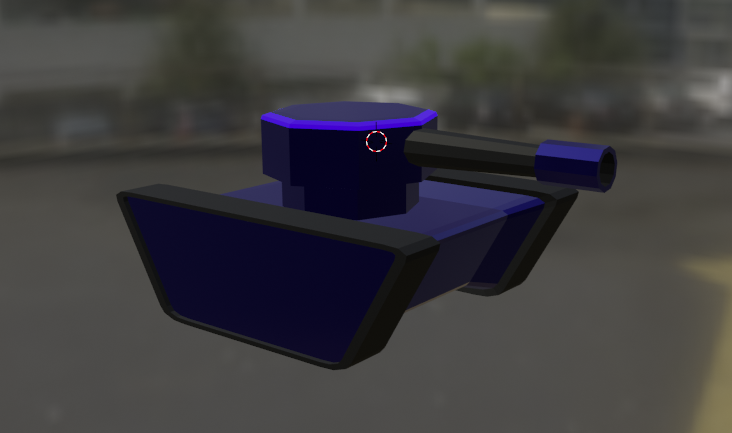
\includegraphics[width=.8\linewidth]{Images/development/model.png}
        \caption{Model w programie Blender.}
        \label{fig:model}
    \end{subfigure}
    
    \begin{subfigure}{.7\textwidth}
        \centering
        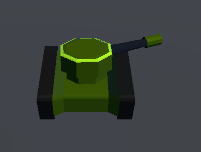
\includegraphics[width=.8\linewidth]{Images/development/model_green.png}
        \caption{Model o programowo zmienionych barwach.}
        \label{fig:model_green}
    \end{subfigure}
    \caption{Model czołgu.}
    \label{fig:both_models}
\end{figure}



\section{Implementacja mechanik}

\section{System sieciowy}

\section{Testy}

\section{Wyniki implementacji}

